% !TEX root = Master.tex


All regression models are fitted using all available covariates: 
\begin{align*}
\text{Diameter} \sim \text{Tree Height} + \text{Crown Area} + \text{factor(Species)}
\end{align*}

\begin{table}[H]
\setlength\arrayrulewidth{1pt}
\centering

\begin{adjustbox}{max width=\textwidth}
\begin{tabular}{|c| c c| c c| c c|}
\hline
\rowcolor{SeaBlue}
 \multicolumn{1}{|c|}{\textbf{Coefficients}} &  \multicolumn{2}{|c|}{\textbf{Log-linear Model}} &  \multicolumn{2}{|c|}{\textbf{GLM Gaussian (Link: Log)}} &  \multicolumn{2}{|c|}{\textbf{GLM gamma (Link: Log)}}  \\
\hline 
\rowcolor{Gray}
\multicolumn{1}{|c|}{-} & \multicolumn{2}{|c|}{Estimate \& Std. Error} & \multicolumn{2}{|c|}{Estimate \& Std. Error} & \multicolumn{2}{|c|}{Estimate \& Std.Error} \\ 
\hline 
Intercept & 1.685 & 0.010 & 1.498 & 0.014 & 1.709 & 0.010 \\ 
\hline 
Height & 0.081 & 0.000 & 0.091 & 0.001 & 0.081 & 0.000 \\ 
\hline 
Crown Area & 0.001 & 0.000 & 0.001 & 0.000 & 0.001 & 0.000 \\ 
\hline 
Art\_ grpDgl & -0.296 & 0.008 & -0.415 & 0.008 & -0.305 & 0.008 \\ 
\hline 
Art\_ grpEi & 0.183 & 0.010 & 0.222 & 0.008 & 0.174 & 0.010 \\ 
\hline 
Art\_ grpFi & -0.185 & 0.009 & -0.259 & 0.009 & -0.195 & 0.009 \\ 
\hline 
Art\_ grpKi & -0.115 & 0.007 & -0.139 & 0.007 & -0.125 & 0.007 \\ 
\hline 
Art\_ grpLä & -0.250 & 0.015 & -0.323 & 0.015 & -0.254 & 0.016 \\ 
\hline 
Overdispersion $\Phi$ & - & - & 12.5 & - & 0.01 & - \\ 
\hline 
\end{tabular} 
\end{adjustbox}

\caption{Diameter prediction models: log-linear, Gaussian and gamma}
\label{tab:Prediction Models}

\end{table}

The estimates in all models (see Table \ref{tab:Prediction Models}) are significantly different from 0. The untransformed confidence
intervals are visualized in Figure \ref{fig:Coefficients}. The transformed confidence intervals for the gamma model are found in
Table \ref{tab:CI}.

\begin{figure}[H]
  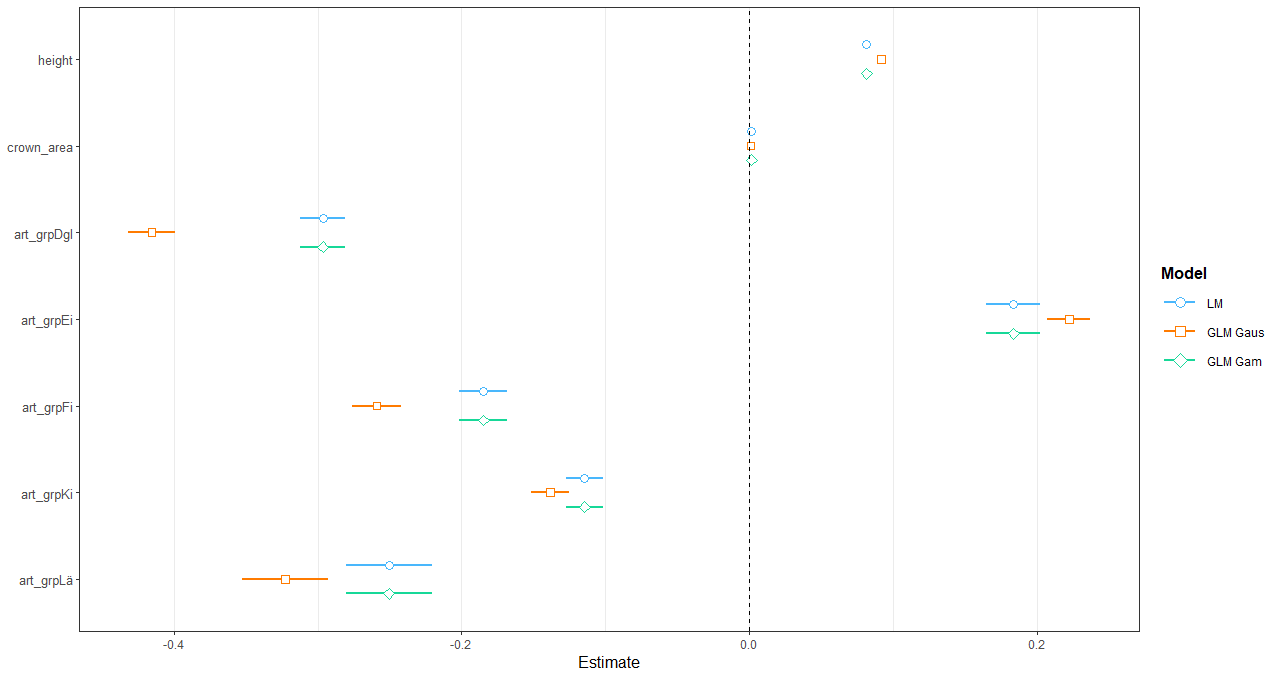
\includegraphics[width=\textwidth]{figures/coefficients.png}
  \caption{While the estimates and confidence intervals of the gamma and log-linear model tend to be similar. The Gaussian model estimates are larger for values greater 0 and smaller for values smaller then 0.}
  \label{fig:Coefficients}
\end{figure}


\begin{table}[H]
\setlength\arrayrulewidth{1pt}
\centering
\begin{adjustbox}{max width=\textwidth}
\begin{tabular}{|c| c| c| c|}
\hline 
\rowcolor{Gray}
\textbf{Coefficient} & \textbf{2.5\% CI Lower bound} & \textbf{97.5\% CI Upper bound} & \textbf{CI Width} \\
\hline
Intercept & 5.4170 & 5.6320 & 0.2150 \\ 
\hline 
Height & 1.0831 & 1.0851 & 0.0020 \\ 
\hline 
Crown Area & 1.0013 & 1.0016 & 0.0003 \\ 
\hline 
Art\_ grpDgl & 0.7250 & 0.7488 & 0.0238 \\ 
\hline 
Art\_ grpEi & 1.1666 & 1.2135 & 0.0469 \\ 
\hline 
Art\_ grpFi & 0.8085 & 0.8375 & 0.0290 \\ 
\hline 
Art\_ grpKi & 0.8704 & 0.8943 & 0.0239 \\ 
\hline 
Art\_ grpLä & 0.7515 & 0.8002 & 0.0487 \\ 
\hline 
\end{tabular} 
\end{adjustbox}

\caption{Transformed confidence intervals (CI) and width of the gamma model in cm}
\label{tab:CI}


\end{table}

Model selection is done by three criterions: R² , AIC \& BIC and Residual Sum of Squares (RSS)
\begin{align*}
\sum{(y - \hat{y_{predict}})^2}.
\end{align*}
\\
All values can be found in Table \ref{Model Selection}.


\begin{table}[H]
\setlength\arrayrulewidth{1pt}
\centering
\begin{adjustbox}{max width=\textwidth}
\begin{tabular}{|c|c|c|c|c|c|}
\hline
\rowcolor{Gray}
\textbf{-}                                                                               & \textbf{LM}       & \multicolumn{2}{c|}{\textbf{GLM Gaussian}} & \multicolumn{2}{c|}{\textbf{GLM gamma}} \\ \hline
\multirow{3}{*}{\begin{tabular}[c]{@{}c@{}}R² / Pseudo R² \\ (Cragg-Uhler)\end{tabular}} & \multirow{2}{*}{} & Null Deviance             & 654900         & Null Deviance            & 533.9        \\ \cline{3-6} 
                                                                                         &                   & Residual Deviance         & 46260          & Residual Deviance        & 35.72        \\ \cline{2-6} 
                                                                                         & 0.937             & \multicolumn{2}{c|}{0.929}                 & \multicolumn{2}{c|}{0.933}              \\ \hline
AIC                                                                                      & -                 & \multicolumn{2}{c|}{19903.18}              & \multicolumn{2}{c|}{19102.88}           \\ \hline
BIC                                                                                      & -                 & \multicolumn{2}{c|}{19959.15}              & \multicolumn{2}{c|}{19158.84}           \\ \hline
RSS                                                                                      & 60136.49          & \multicolumn{2}{c|}{46257.25}              & \multicolumn{2}{c|}{53569.47}           \\ \hline
RSE ($\sqrt{RSS/n}$)                                                                                  & 4.0315            & \multicolumn{2}{c|}{3.53581}               & \multicolumn{2}{c|}{3.80503}            \\ \hline
\end{tabular}
\end{adjustbox}

\caption{Model selection criterion for Log-linear, Gaussian and gamma}
\label{Model Selection}
\end{table}

The models have a (pseudo) R² of almost 93\% while the Log-linear model is favorable with 93.7\% explained variation. The AIC \& BIC of the gamma model is better compared to the Gaussian model. This cannot be compared to the Linear Model, of which the AIC is constructed based on the RSS and not a likelihood. Finally, the Gaussian model has the lowest Sum Squares and therefore the smallest Residual Standard Error with approximately 3.53 cm in the diameter.\\

All models have an exceptional fit, whereby we finally decide to use the gamma model. A bias correction
is introduced by fitting parametric distributions in Section \ref{Distribution Engineering}. Thus, the model with the highest likelihood (AIC \& BIC) is finally favoured.\\

Figure \ref{fig:Pane} visualizes the good fit of the model. Most points by species are well described by the panes, whereby
we see for both tree species an underestimation at large value. This is expected, as trees have natural high
limits. Once it is reached, only the diameter increases, resulting in the underestimation. \\

\begin{figure}[H]
  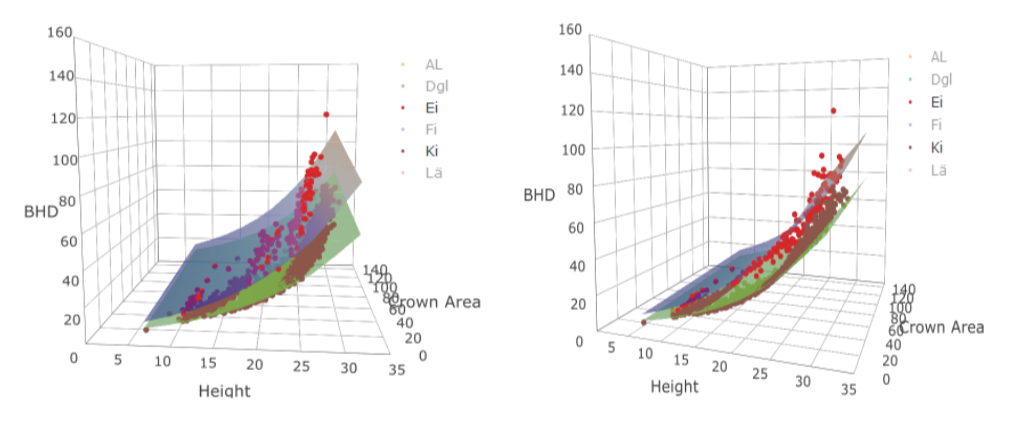
\includegraphics[width=\textwidth]{predicted_pane.png}
  \caption{Predicted pane of the gamma model for oaks (Ei red) and pines (Ki brown)}
  \label{fig:Pane}
\end{figure}

Figure \ref{fig:Residuals GLM gamma} displays the residual plots of the gamma model. Some unwanted behavior is seen in the scale location
plot, which is used to identify violations of homoscedasticity. A somewhat linear behavior between 2.5 to 3
followed by a curvature to 4 results in potential mild heteroskedasticity for larger values as indicated by the red
line. 5 unique observations in over 3700 observations
are identified as outliers. This leads to the conclusion that the GLM gamma fits well and is acceptable regarding
the underlying assumptions.

\begin{figure}[H]
  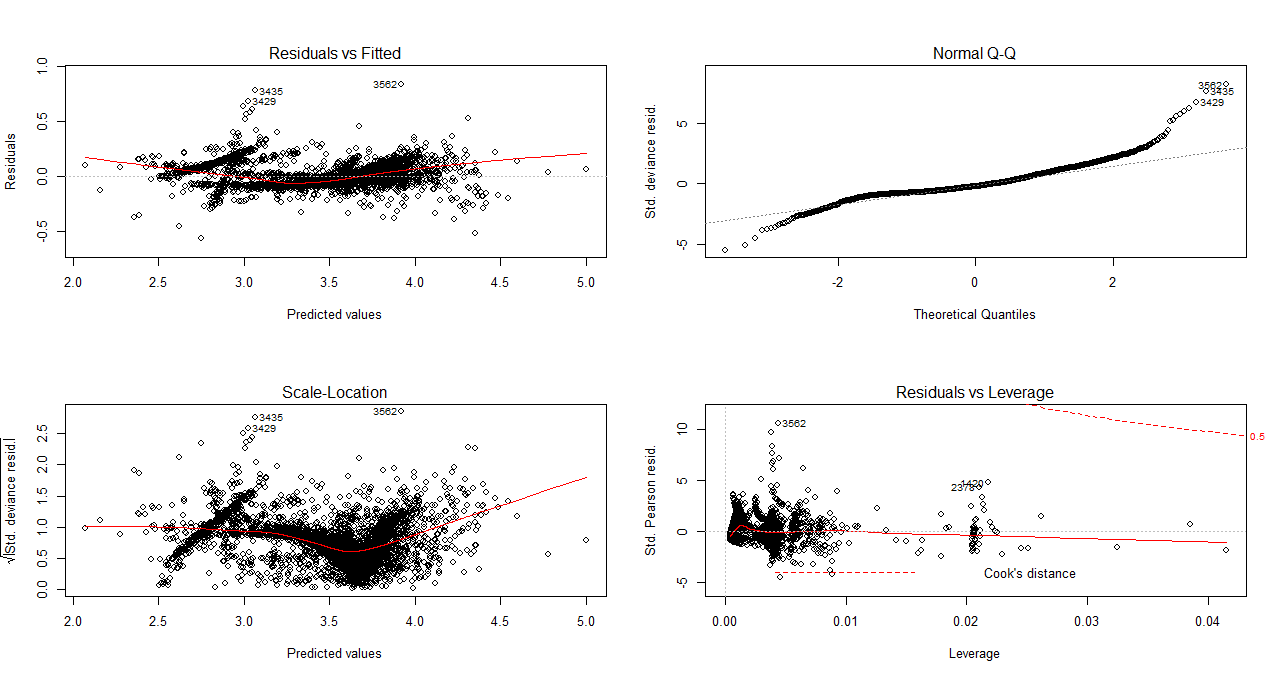
\includegraphics[width=\textwidth]{residuals_glm_gamma.png}
  \caption{Residual plots of GLM gamma. Data points with an index are considered outliers.}
  \label{fig:Residuals GLM gamma}
\end{figure}
